% Chapter 4

\chapter{Deoptimization in RJIT} % Main chapter title

\label{Chapter4} % For referencing the chapter elsewhere, use \ref{Chapter4} 

%----------------------------------------------------------------------------------------

% Define some commands to keep the formatting separated from the content 
\newcommand{\keyword}[1]{\textbf{#1}}
\newcommand{\tabhead}[1]{\textbf{#1}}
\newcommand{\code}[1]{\texttt{#1}}
\newcommand{\file}[1]{\texttt{\bfseries#1}}
\newcommand{\option}[1]{\texttt{\itshape#1}}

%----------------------------------------------------------------------------------------
This chapter presents our design to support OSR transitions and OSR deoptimizations in LLVM, and more particularly in the RJIT project.
Our design and implementation is based on OSR Kit\cite{OSRKit, OSRKitGit}, an OSR library for LLVM, implemented by \citean{OSRKit} at the department of Computer, Control, and Management Engineering of the Sapienza University of Rome.
This implementation provides several features of existing techniques, that were never simultaneously supported in a single framework.
It is flexible enough to be used to implement our own model for OSR deoptimization.
We therefore decided to use and extend it, in order to provide OSR deoptimization for R.\\

\section{Overview}
This section presents our goals for this Master Thesis Project and justifies the use of the OSR Kit as the base of our OSR support in RJIT.\\

%TODO MAYBE switch the Justification and the LLVM Library

\subsection{Justification}
%Our goal: OSR deoptimization for R.
    %R has shitty performances
    %need aggressive optimizations
    %Work with the rjit project, so based on LLVM. 
    %Too soon to know what we really want, so need a mechanism as flexible as possible.
%What do we want form OSR Kit? 
    %A transition mechanism
    %An LLVM library that is mostly optimization and language independent.
        %Why? Because we want to work at the LLVM IR level, which is stable.
%Why not from scratch?
    %Reinventing the wheel seems like a waste of time. 
    %Enables to focus on deoptimization case.
    %Enables to test a proper optimization. 
    %Can extend it with new features, can modify it.
The goal of this Master Thesis project is to provide a flexible OSR deoptimization framework in LLVM, and use it to improve performances in RJIT, our LLVM JIT compiler for R.
R is a programming language and software environment for the statistical computing and graphics, developed by the R Foundation for Statistical Computing\cite{RURL}.
Due to SAY WHYYYYYYYYYYYYYYYYYYYYYYYYYY OOOOOHHHHH GOOOOOOODDDDDD WHHHYYYYYYYYYY, R exhibits very poor performances CITE SOMETHING.
The RJIT project strives to improve these performances by providing a LLVM based JIT compiler for R. SAY MORE.
The RJIT compiler is still pretty young, only a few months old.
As a result, we lack FEEDBACK; DONT KNOW EXACTLY HOW TO IMPROVE PERF AND NEED TO EXPERIMENT.
Therefore, we are looking for a flexible and extensible OSR mechanism that enables us to prototype and experiment various solutions, without trapping ourselves into a single model.\\

The OSR Kit library\cite{OSRKit} is a flexible implementation of on-stack replacement instrumentation in LLVM.
The source-code for the library is available on Github\cite{OSRKitGit}, and the library can be used in any LLVM project by simply copy-pasting the OSR Kit files inside of it.
The simple integration, the availability of the source code, and the flexibility of the framework make it a perfect base implementation upon which we can implement our support for OSR deoptimization mechanisms in RJIT.\\

%TODO MORE ABOUT THE FOCUS ON DEOPT.
This master project thesis focuses on the design and implementation of a prototype for OSR deoptimization support in RJIT.
Starting a new OSR transition implementation from scratch requires time.
Using a flexible and modifiable OSR transition library therefore seemed like the goto option.
We do not waste time reimplementing something that already exists, and can therefore put all our efforts into implementing an interesting OSR deoptimization case, testing it, and extending the OSR Kit library with mechanisms that are specific to our needs (Sections \ref{osrForUs} and \ref{extendingOSR}).\\

\subsection{An LLVM Library}

The OSR Kit is a general-purpose, target-independent, implementation of on-stack replacement for LLVM.
As such, it can be used by any LLVM based compiler.
The main goals of the OSR Kit project are:
\begin{enumerate}
    \item To allow chained OSR transitions, i.e., a continuation function can be instrumented to allow OSR transitions.
    \item To support OSR entries and exits via the same instrumentation.
    \item To allow transitions at arbitrary function locations.
    \item To allow continuation functions to be either generated at run time, or already known at compilation time (i.e., generated on the fly or cached).
    \item To encapsulate and hide the OSR implementation details from the front-end.
    \item To encode OSR transitions entirely at the LLVM IR level.
    \item To limit the intrusiveness of the OSR instrumentation.
    \item To allow the LLVM's compilation pipeline to generate the most efficient native code for an instrumented function. \label{llvmTransformPasses}
\end{enumerate}

%2 means that what the framework really provides is a transition mechanism. 
%3 leaves the responsability to the user to id potential transition points
%4 we have both the generated on the fly and the cached semantics, enables us to test both.
%6 Stable representation
%8 This point is important in our case study Chapter 5, inlining mostly to extend the scope of possible optimizations.
%MORE about it being a tool and the OSR is left to the user.
The OSR Kit library's main contribution is the implementation of an efficient and flexible OSR transition mechanism.
This transition can be used to implement OSR entries and OSR exits alike.
Allowing OSR points to be inserted at any location enables the user to experiment the OSR mechanisms at any instruction boundary. 
In other words, the OSR library is designed to give the user as much freedom as possible.
Section \ref{tradeOffs} explained the basic trade-offs between generating the continuation function on the fly and caching already compiled versions.
Where other implementations, such as McJIT OSR\cite{lameed2013modular}, made a clear choice between the two techniques, the OSR Kit library decided to enable both of them, hence allowing the user to experiment and select the design that better suits specific use cases.\\

LLVM IR is a stable representation that combines the advantages of both the high-level representation, i.e., it still contains some semantic constructions particular to the language being compiled, and the advantages of a lower level representation, closer to the execution engine.
In the case of this master thesis project, i.e., providing OSR mechanisms in the RJIT project, the LLVM IR is the exact middle layer representation that we need. 
The R AST representation is too high level and prevents us from introducing efficient OSR instrumentation. 
At the LLVM IR level, the R semantics are still visible and it therefore allows us to efficiently implement our optimizations.\\

Point \ref{llvmTransformPasses} is important in order to leverage the full power of the LLVM transformation and optimization passes.
One of the main advantages of using the LLVM framework is that LLVM transformation passes and optimizations can be automatically added to the compilation pipeline in order to improve the quality of the code generated.
For example, in the case study in Chapter \ref{Chapter5}, one of the OSR inlining mechanism's goals is to extend the scope in which the LLVM passes run in order to improve the code quality.\\


\section{Resolved \& Open OSR}
The OSR Kit library\cite{OSRKit} provides the choice between generating the continuation function of an OSR transition on the fly, or using an already compiled function.
This section describes both techniques as they are implemented in the OSR Kit library.\\
 
\subsection{The Open OSR}
%Generate on the fly.

%How it works
    %theory
    %practice

%Ok for optimizations
%Less okay for deoptimization.
The \textit{open OSR} scenario corresponds to the case where the continuation function is generated when the OSR transition is fired.
Deferring the compilation of the continuation function allows profiled-guided compilation strategies to gather as much information as possible about the current state of the execution, and therefore generate the best possible code.\\

The open OSR scenario is implemented as a call to a stub function, call it $f_{stub}$.
The $f_{stub}$ function is responsible for generating the continuation function, and then transferring the execution to it.
The continuation function is generated by a special \textit{gen} function, that takes as inputs the base function $f$, i.e., the from function, and the OSR point that triggered the transition.\\
%TODO code for the OSR points open. 

Figure REF corresponds to the signature of the OSR Kit function that enables to insert open OSR points.
The \textit{destFunGenerator} is the $f_{stub}$ function and is of type \textit{DestFunGenerator}, described in Figure REF.\\

\begin{minipage}{\linewidth}
\includecode{Code/DestFunGenerator.c}
\end{minipage}

\begin{minipage}{\linewidth}
\includecode{Code/OpenOSR.c}
\end{minipage}

Open OSR are hard in the deoptimization case.
Being able to generate a continuation function on the fly for an OSR exit requires the framework to be able to undo an optimization.
The RJIT framework, does not, for the moment, provide means to keep track of transformations performed on a function, and efficiently revert them.
For example, the VARMAP data structure in the Jikes RVM OSR implementation\cite{soman2006efficient} is automatically updated by the framework when a transformation is performed on the function.
This enables to reverse the steps that lead to the optimized version.
While the RJIT compiler does not provide such mechanism, we could imagine keeping the LLVM IR of the original function in memory, without compiling it.
When an open OSR exit is triggered, the unoptimized LLVM IR for the function is retrieved, the continuation point is identified, and RJIT instruments and compiles the correct continuation function.
This solution enables to avoid the cost of going through the entire compilation of the continuation function until it is truly needed.
On the other hand, it increases the amount of work performed during the OSR transition.\\
%TODO add a sentence to say if it is tested or not in our implementation
%In order to do so, we have a handler, that keeps the version etc., 
%So I guess I'm gonna try it.

\subsubsection{Similarities with McJIT}
The open OSR is similar, in theory, to the McJIT OSR implementation\cite{lameed2013modular}.
Both of them rely on a \textit{gen} function to generate the continuation function when the OSR transition is fired.
However, \citean{OSRKit} made the choice to perform these operations, i.e., generating the continuation function and transferring the execution, inside a separated function, rather than instrumenting the from function directly.
This choice was made in order to minimize the code injected inside the from function.
In fact, the instrumentation, even when inserted in a separated branch, might interfere with compiler optimizations.
Examples of such interferences are the increase of register pressure, the alteration of code layout and instruction cache behavior.\\

\subsection{The Resolved OSR}

The \textit{resolved OSR} scenario corresponds to the case where the continuation function is known prior to fire the OSR transition, and the from function has been instrumented to transfer the execution to this specific continuation function.
In the resolved OSR scenario, the transition is expected to be faster than in the open scenario, since there is no compilation to be performed. 
This technique also enables to reuse functions that were compiled previously, e.g., either because several from functions have the same continuation function, or because an OSR point is fired several times during the execution of the program.\\

The resolved OSR is implemented as a call to the continuation function, which takes as inputs all the live variables at the OSR point as inputs.
The continuation function is instrumented to jump at the correct location inside the code to resume the execution. 
Figure \ref{ResolvedOSRFig} illustrates the resolved OSR scenario.\\

\begin{figure}[h]
\centering
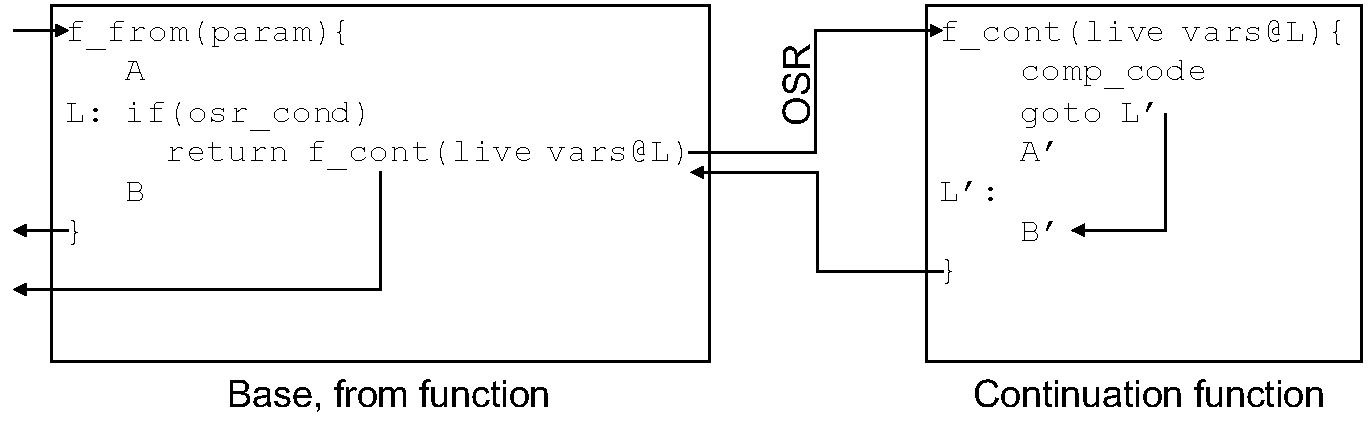
\includegraphics[scale=0.5]{Figures/OSRKitResolvedScenario}
\decoRule
\caption[Resolved OSR Scenario]{Resolved OSR scenario, from\cite{OSRKit}.}
\label{ResolvedOSRFig}
\end{figure}

Figure REF corresponds to the signature of the OSR Kit function that enables to insert resolved OSR.\\

\begin{minipage}{\linewidth}
\includecode{Code/ResolvedOSR.c}
\end{minipage}

The resolved OSR scenario does not require to inverse on the fly the transformations performed on the function and can therefore easily be used to implement the deoptimization case.
In order to obtain the optimized version of a function, one has to perform transformations on a base function.
This base function can therefore be used as the continuation function in the case of an OSR exit.
In RJIT, we rely on the resolved OSR to provide deoptimization of functions where call sites were inlined.
While generating the optimized version by speculatively inlining calls, the RJIT compiler introduces the OSR exit instrumentation with the base function as continuation function.
When several call sites are inlined, each of them is instrumented with an OSR exit that points to its own continuation function, which is a copy of the base function with the proper OSR instrumentation (see Section \ref{thecontinuationfunction}).\\



\section{The API}
\subsection{OSR Points \& Conditions}
%No distinction
%Both are done in the same way i.e., insert a condition.
%Do the condition testing, do the jump to a special block.
%Requirements for the point to be inserted !

In the OSR Kit library\cite{OSRKit}, there is no distinction at the implementation level between OSR exits and entries.
The general mechanism used is the OSR point.
An OSR point corresponds to a labelled LLVM basic-block that contains the call to the continuation function and the return instruction to propagate the result of the call.
OSR points are protected by an OSR condition. 
The OSR Kit library allows an OSR condition to be any vector of LLVM instructions. 
The last instruction is automatically used by the framework as condition for an LLVM branch instruction. 
If the condition succeeds, the OSR transition is fired.
Otherwise, the execution continues in the function.\\

Figures REF and REF provide an example of OSR instrumentation.
In Figure REF, we have the R declaration of two functions, $f$ and $g$, and the simplified LLVM IR generated for $g$ in RJIT.
Figure REF presents the instrumented version of $g$, in which an OSR point has been inserted.
Lines 5 and 6 correspond to the OSR condition.
In this example, the OSR is fired if the line 1 does not yield the same function for $f$ as the one that was used by the RJIT compiler when it generated the instrumented function.
If the OSR is fired, the execution jumps to the \textit{OSR\char`_fire} basic block and calls the continuation function, namely \textit{OSRCont}.
The OSR point \textit{OSR\char`_fire} calls the continuation and propagates its return value line 15.
The \textit{OSR\char`_split} block corresponds to the regular continuation of the function $f$ when the OSR is not fired.\\

\begin{minipage}{\linewidth}
\includecode[asm]{Code/original.llvm}
\end{minipage}

\begin{minipage}{\linewidth}
\includecode[asm]{Code/fromInstrumented.llvm}
\end{minipage}

\subsection{The StateMap}
\subsection{The continuation function}\label{thecontinuationfunction}

\section{Using OSR Kit to deoptimize}\label{osrForUs}
\subsection{The unease of deoptimizing}
\subsection{SOMETHING}
\subsection{SOMETHING ELSE}

\section{Extending OSR Kit}\label{extendingOSR}
\subsection{Handling versions}
%Updating the statemap as we perform the operations.
\subsection{Unguarded OSR points}
\subsection{Fusing versions?}
%TRANSITIVE STATEMAPS